\documentclass{article}

\usepackage{polski}
\usepackage[utf8]{inputenc}
\usepackage{graphicx}
\usepackage{url}
\usepackage{amsmath}

\usepackage{float}

\newcommand{\bb}{\textbf}


\title{Sieci neuronowe i neurosterowniki}
\date{2017-11-27}
\author{Jędrzej Kozal, Michał Leś}

\begin{document}

\begin{titlepage}
	\centering
	
\includegraphics[width=0.25\textwidth]{logo_pol_wroclaw.png}\par\vspace{1cm}
	{\scshape\LARGE Politechnika Wrocławska \par}
	\vspace{1cm}
	{\scshape\Large Sieci neuronowe i neurosterowniki \par}
	\vspace{1.5cm}
	{\huge\bfseries Sprawozdanie z projektu \par}
	\vspace{2cm}
	{\Large\itshape Michał Leś, Jędrzej Kozal\par}
	\vfill
	prowadzący\par
	Dr inż. ~Piotr \textsc{Ciskowski}

	\vfill

% Bottom of the page
	{\large 2017-10-01\par}
\end{titlepage}

\section{Wstęp}
Podstawowym założeniem projetku jest zaznajomienie się z neurosterownikami, ich zasadami działania oraz przygotowanie modelu predykcyjnego prostego obiektu dynamicznego. Dodatkowo przyjęto że bardziej interesujące będzie przyjęcie jakiegoś rzeczywistego obiektu niż badanie reakcji bardziej teoretycznego modelu o przyjętych charakterystykach.

Neurosterowniki są sposobem zaadresowania w automatyce kwestii sterowania obiektami mocno nieliniowymi, z którymi tradycyjne metody sterowania jak sterowniki PID nie dają sobie rady. U podstaw działania neurosterowników leży idea działania sieci neuronowej, które ostatnio zdominowały pole uczenia maszynowego. Są one wykorzystywane w wielu dziedzinach nauki i techniki do rozpoznawania obrazów (computer vision), klasyfikacji, sterownia ruchem ulicznym, wspomagania użytkowników różnych aplikacji (jak np. podpowiadanie słów w trakcie pisania na smartphonie), czy nawet prowadzenie eksperymentów społecznych. W niniejszej pracy postawiono zbadać w jaki sposób szerokie możliwości oferowane przez sieci neuronowe mogą być wykorzystane w automatyce.

\section{Podstawy teoretyczne}

\subsection{Przyjęty model obektu}

Obiekt w automatyce jest traktowany jako czarna skrzynka, która posiada wejścia i wyjścia. Na pobudzenie na wejściu reaguje odpowiedzią na wyjściu. Odpowiedź systemów dynamicznych zależy nie tylko od aktualnej wartości wejścia, ale także od stanu obiektu w poprzednich chwilach. Zgodnie z tym można zapisać model nieliniowego dyskretnego obiektu dynamicznego jako:

\begin{equation}
\left\{
\begin{array}{ll}
	\bb{x}(k+1) &= \phi (\bb{x}(k), \bb{u}(k)) \\
	\bb{y}(k)   &= \psi (\bb{x}(k))
\end{array} \right.
\label{rownanie_stanu}
\end{equation}

Układ \ref{rownanie_stanu} przedstawia równania stanu. Pierwsze równanie wiąże wewnętrzny stan obiektu z pobudzeniem, a drugie równanie wiąże stan obiektu z wyjściem. System opisywany tymi równaniami jest niezmienny w czasie (angl. time-invariant) - $\phi$ i $\psi$ nie zależą bezpośrednio od czasu.

Jeśli zastąpimy funkcje nieliniowe przez odpowiednie macierze zyskamy system liniowy:

\begin{equation}
\left\{
\begin{array}{ll}
	\bb{x}(k+1) &= A\bb{x}(k) + B\bb{u}(k) \\
	\bb{y}(k)   &= C\bb{x}(k) + D\bb{u}(k)
\end{array} \right.
\end{equation}

W rzeczywistych systemach w równaniach oprócz stanu $\bb{x}$ i pobudzenia $\bb{u}$ pojawiają się także zakłócenia $\bb{z}$, które nie będą tutaj rozważane.

Klasa systemów liniowych jest od dawna dobrze znana. Znaleziono wiele sposobów badania i algorytmów sterowania obiektami liniowymi. O wiele trudniejsze w sterowaniu są obiekty nieliniowe. Nawet znając funkcję $\psi$ oraz $x(k)$ samo stworzenie modelu mogącego dokonać identyfikacji takiego obiektu jest trudne, ze względu na kumulujące się z czasem błędy numeryczne, oraz poprzez konieczność poczynienia założeń co do stabilności systemu.

Najprostsza reprezentacja systemu dynamicznego nie zawiera wewnętrznego stanu, który w wielu przypadkach może być pominięty

\begin{equation}
	\bb{y}(k+1) = f(\bb{y}(k),\bb{u}(k))
\end{equation}

\subsection{Zadanie identyfikacji obiektu}

Zadanie identyfikacji sprowadza się do wyznaczeniu modelu reagującego na pobudzenie w sposób zbliżony do reakcji rzeczywistego obiektu:

\begin{equation}
	|| \hat{y} - y || < \epsilon
	\label{warunek}
\end{equation}

\begin{figure}
\centering
	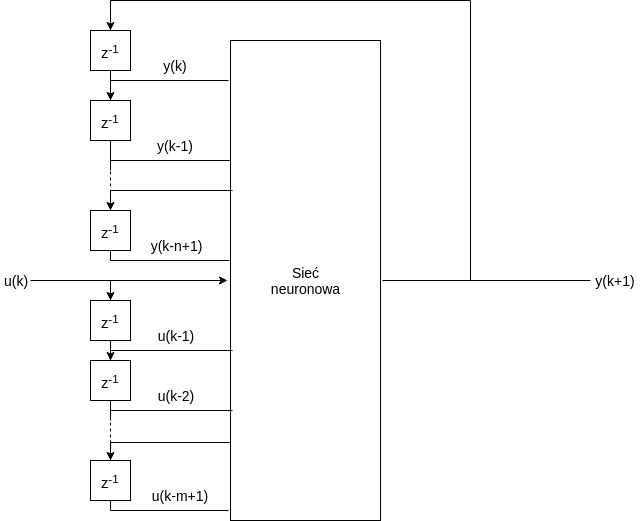
\includegraphics[width=0.90\textwidth]{ident.jpg}\par\vspace{1cm}
\caption{Model identyfikacji obiektu z wykorzystaniem sieci neuronowej.}
	\label{fig:identyfikacja}
\end{figure}

Uzyskanie takiego modelu umożliwia sterowanie adaptacyjne, co znacznie ułatwia pracę z obiektami nieliniowymi. Celem sterowania w ogólności jest uzyskanie na wyjściu obiektu $\bb{y}(k)$ wartości jak najbardziej zbliżonej do wartości zadanej $\bb{y}_m(k)$. W przypadku sterowania adaptacyjnego oznacza to znalezienie takiego pobudzenia $\bb{u}(k)$ aby została spełniona zależność:

\begin{equation}
	\displaystyle{\lim_{k \to \infty}} ||\bb{y}(k)-\bb{y}_m(k)|| < \epsilon
\end{equation}

Często do takiego zadania są wykorzystywane sieci neuronowe przedstawione na rys. \ref{fig:identyfikacja}. Na wejście sieci podaje się wejścia systemu, oraz wyjścia z poprzednich chwil. Zadaniem sieci jest przewidzenie zachowania systemu w kroku $k+1$. Szereg bloków opóźniających będzie dalej oznaczany w pracy jako TDL(Tapped Dleay Line).

\begin{figure}
\centering
	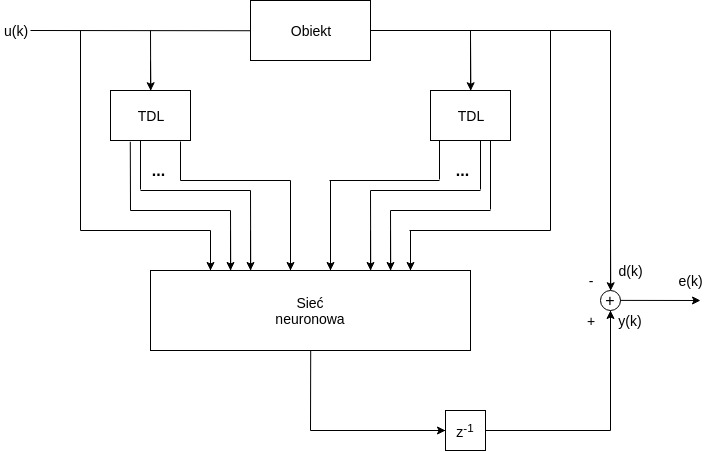
\includegraphics[width=0.90\textwidth]{ident2.jpg}\par\vspace{1cm}
\caption{Schemat podłączenia sieci neuronowej w trakcie uczenia.}
	\label{fig:identyfikacja2}
\end{figure}

W trakcie identyfikacji sieć neuronowa jest zwykle włączana sposób szeregowo-równoległy, co zostało zilustrowane na rys \ref{fig:identyfikacja2}. Taka konfiguracja umożliwia badanie błędu i minimalizację błędu zgodnie z nierównością \ref{warunek}. Sieć neuronowa nieustanie próbuje przewidzieć wyjście obiektu w następnej chwili. Różnica $e(k)$ jest wykorzystywana w procesie uczenia sieci. W \cite{Osowski} zaproponowano taką metodę oraz zaprezentowano wykorzystanie modelu do predykcji wyjścia filtru Butterwortha szóstego rzędu dla pobudzenia sygnałem trójkątnym oraz tłumionym sygnałem sinusoidalnym.
\newpage
\section{Zrealizowane zadania oraz otrzymane wyniki}
Zadanie predykcji może zostać zrealizowane za pomocą modelowania liniowego ARX -
modelu auteregresywnego z zewnętrznym wejściem. Jeżeli do modelowania zostały
użyte sieci neuronowe model taki nazywa się NNARX (Neural Network ARX).


Zadanie zostało podzielone na dwie części - pierwsza część zakłada użycie domyślnych
narzędzi do tworzenia sieci neuronowych w środowisku Matlab. Wymaga to nieco więcej
nakładu w przygotowaniu zbiorów uczących i zarządzania sieciami.
Druga metoda opiera się na zastosowaniu specjalnego dodatku do Matlaba służącego
do tworzenia modelów liniowych ARX za pomocą sieci neuronowych (toolbox NNARX).


Na podstawie danych zawartych w pliku 'actuator.m' żądany model został załadowany
do środowiska programu Matlab. Wejściem obiektu (u) jest
otwarcie zaworu, zaś odpowiedzią systemu(y) jest ciśnienie oleju.

\begin{figure}[H]
\centering
	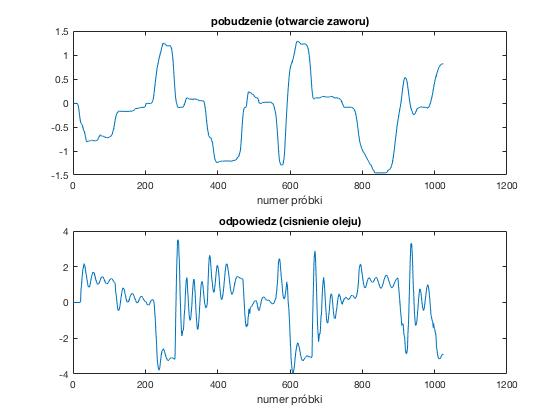
\includegraphics[width=0.70\textwidth]{data.jpg}
\caption{Dane wejściowe zależne od czasu}
	\label{fig:data}
\end{figure}

Pierwszym elementem potrzebnym do wykonania zadania była konstrukcja prawidłowego ciągu uczącego.
W modelu ARX potrzebujemy stworzyć układ z opóźnionymi wejściami i odpowiedziami.
W zależności od potrzeb modelu, możemy dostosować wielkość opóźnienia i ilość opóźnionych próbek.
W naszym przypadku skonstruowana została następującą macierz wejściowa dla sieci:
\label{eq:us}
\begin{equation}
	u_s= \begin{bmatrix} 0 & 0 & 0 & 0 \\ 0 & u' & 0 & 0 \\ 0 & 0 & u' & 0 \\ 0 & p' & 0 & 0 \\ 0 & 0 & p' &  0 \\ 0 & 0 & 0 & p' \end{bmatrix}
\end{equation}
gdzie u' i y' odpowiadają transponowanym wektorom otrzymanym z modelu.
Analogicznie skonstruowany został wektor pożądanych wyjść dla sieci:
\begin{equation}
	y_s= \begin{bmatrix} p' & 0 & 0 & 0  \end{bmatrix}'
\end{equation}

Dane zostały pogrupowane na zbiór uczący (pierwsze 512 próbek), oraz
zbiór sprawdzający(kolejne 512 próbek).

Tak przygotowane dane zostały poddane procesowi uczenia przyrostowego.
Przykładowe wartości dla minimalnego błędu kwadratowego (MSE) wahały się w okolicach
0.01 co widać na rysunku \ref{fig:25_epoches}.

\begin{figure}[H]
\centering
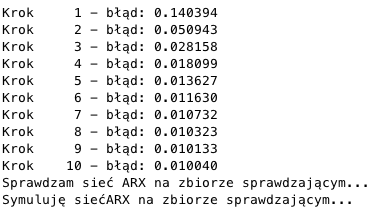
\includegraphics[width=0.60\textwidth]{errors.png}
\caption{Przykładowe wartości błędów}
	\label{fig:error}
\end{figure}

\begin{figure}[H]
\centering
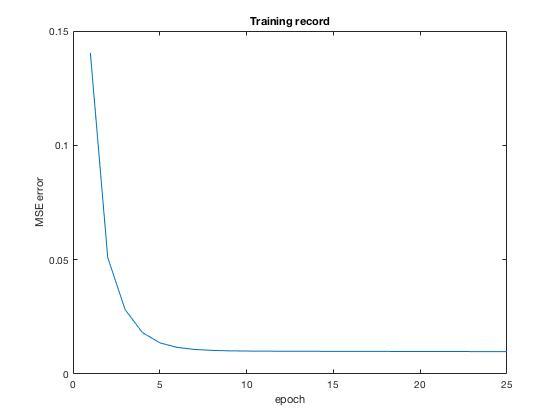
\includegraphics[width=0.60\textwidth]{25_epoches.jpg}
\caption{Zależność błędu od ilości epok}
	\label{fig:25_epoches}
\end{figure}

%
Wraz ze wzrostem ilości epok błąd malał bardzo wolno - na rysunku nr \ref{fig:25_epoches}
jest dobrze widoczne, że  już po 10 epokach otrzymane zostały wartości błędu rzędu błędu po 25 epokach.

Wykresy przedstawione na rysunku \ref{fig:25} przedstawiają testy otrzymanej sieci neuronowej.
W pierwszych dwóch przypadkach dokonano sprawdzenia działania sieci na zbiorze uczącym oraz walidacyjnym
za pomocą metody one-step-ahead. Metoda ta próbuje przewidzieć wyjście obiektu w następnym dyskretnym kroku
na podstawie pełnej informacji o wyjściu obiektu i jego wejściu w przeszłości. Ostatni wykres przedstawia
symulację obiektu za pomocą modelu stworzonego na podstawie sieci. Model ten
powinien modelować badany wcześniej obiekt. Na wykresie widzimy, że zachowanie obiektu modelowanego
w ten sposób jest podobne do rzeczywistego, jednak jest on mniej podatny na wykrywanie zmian.

\begin{figure}
\centering
	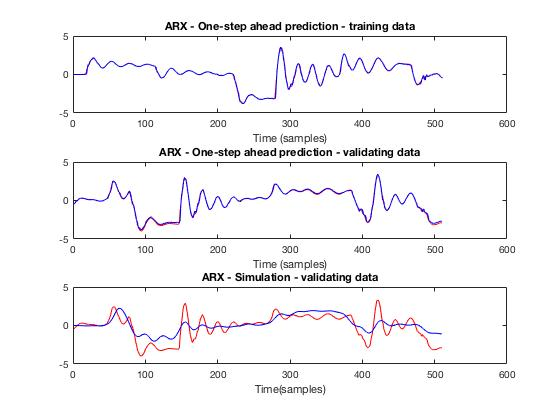
\includegraphics[width=\textwidth]{25}
\caption{Wykresy predykcji one-step-ahead dla zbioru uczącego i walidacyjnego oraz symulacja obiektu}
		\label{fig:25}
\end{figure}

Druga część zadania polegała na stworzeniu modelu za pomocą toolboxa zawierającego
gotowe rozwiązania dla sieci typu NNARX.
Stworzono nowy obiekt zawierający te same dane, oraz załadowano je do niego.
Bardzo wygodną opcją modelowania za pomocą obiektu nnarxnet jest możliwość łatwej
manipulacji wielkością opóźnień wejść i wyjść dla uczenia sieci. W poprzednim
modelu opóźnienia były generowane już na poziomie przygotowania danych do uczenia,
co wymagało nakładu w postaci modelowania wejścia i wyjścia (rysunek \ref{eq:us} na stronie \pageref{eq:us}).
Sieci te są również szybsze w działaniu.
Przy użyciu mechanizmów optymalizacyjnych Matlaba przetwarzanie tych samych
struktur w połączeniu z metodą uczenia Levenberga Marquardta pozwala na uzyskanie
znacznie lepszych efektów.

\newpage
W trybie uczenia sieci (rysunek \ref{fig:open}), przyjmuje ona wejścia pochodzące od prawdziwego obiektu.
\begin{figure}[H]
\centering
	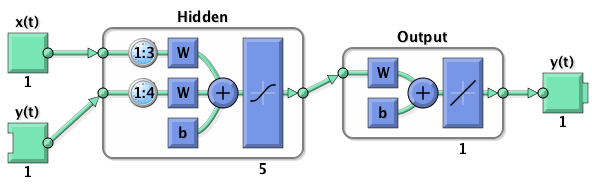
\includegraphics[width=\textwidth]{open.png}
\caption{Schemat sieci NNARX dokonującej predykcji pochodzącej z rzeczywistego obiektu}
		\label{fig:open}
\end{figure}

Jeżeli badany model ma służyć do identyfikacji obiektu (rysunek \ref{fig:closed}), wprowadzenie sprzężenia
zwrotnego spowoduje zachowanie się wyjścia dokładnie tak jak obiekt

\begin{figure}[H]
\centering
	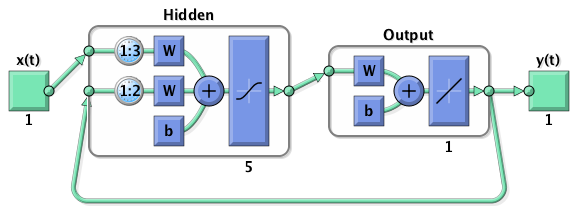
\includegraphics[width=\textwidth]{closed.png}
\caption{Schemat sieci NNARX symulującej obiekt}
		\label{fig:closed}
\end{figure}

Sieć otrzymana w wyniku działania na obiekcie nnarx jest siecią wielowarstwową,
można dzięki temu za jej pomocą łatwo manipulować ilością neuronów w warstwie ukrytej
(szybki czas przetwarzania pozwala na eksperymentowanie z długością uczenia i ilością neuronów
w celu osiągnięcia żądanej dokładności modelu).
Toolbox Matlaba udostępnia bardzo wiele statystyk na temat procesu uczenia i analizy sieci.
Głównym interesującym nas wykresem jest skuteczność metody predykcji typu one-step-ahead
oraz symulacja obiektu czyli poprawność wykonania zadania identyfikacji.

\newpage
Dla 5 neuronów w warstwie ukrytej, 1000 epokach uczenia i opóźnieniem
wejść o 2 i wyjść o 3 na wejściu sieci otrzymałem wykresy przedstawione
na rysunku \ref{fig:5_one_step_ahead}.
Wygenerowanie symulacji obiektu wynikające z zamknięcia pętli sprzężenia zwrotnego
zostało przedstawione na rysunku \ref{fig:5_simulation}.

\begin{figure}[H]
\centering
	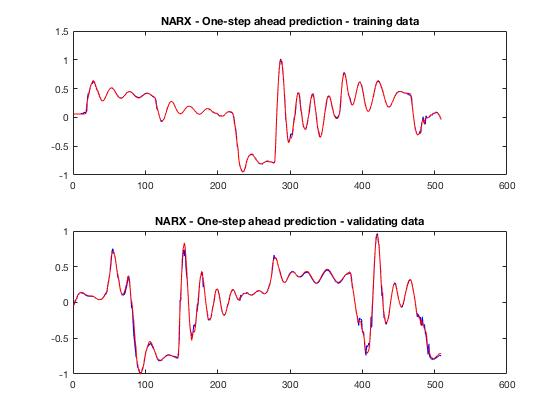
\includegraphics[width=0.80\textwidth,keepaspectratio]{5_one_step_ahead.jpg}
\caption{Wykresy predykcji one-step-ahead dla zbioru uczącego i walidacyjnego}
		\label{fig:5_one_step_ahead}
\end{figure}

\begin{figure}[H]
\centering
	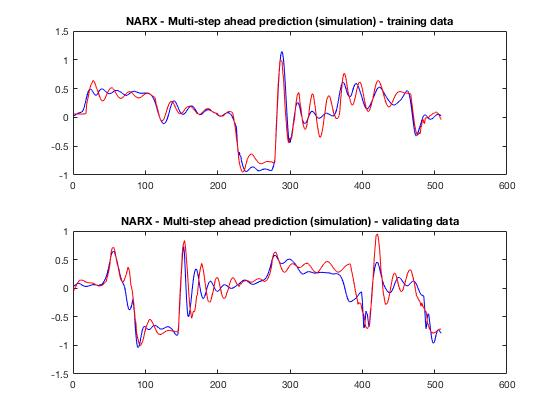
\includegraphics[width=0.75\textwidth,keepaspectratio]{5_simulation.jpg}
\caption{Symulacja rzeczywistego obiektu}
		\label{fig:5_simulation}
\end{figure}



Dla 10 neuronów w warstwie ukrytej, 1000 epokach uczenia i opóźnieniem
wejść o 2 i wyjść o 3 na wejściu sieci otrzymałem wykresy przedstawione
na rysunku \ref{fig:10_one_step_ahead}.
Wygenerowanie symulacji obiektu wynikające z zamknięcia pętli sprzężenia zwrotnego
zostało przedstawione na rysunku \ref{fig:10_simulation}.

\begin{figure}[H]
\centering
	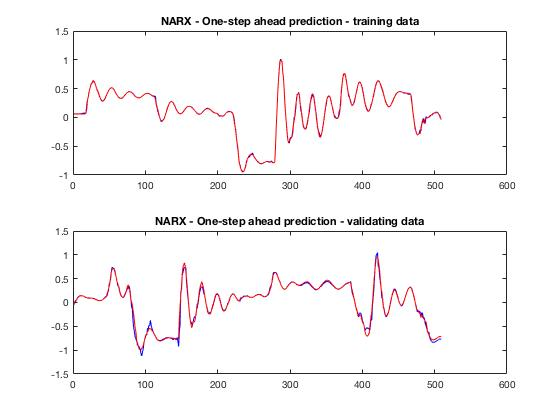
\includegraphics[width=0.80\textwidth, keepaspectratio]{10_one_step_ahead}
\caption{Wykresy predykcji one-step-ahead dla zbioru uczącego i walidacyjnego}
		\label{fig:10_one_step_ahead}
\end{figure}
\begin{figure}[H]
\centering
	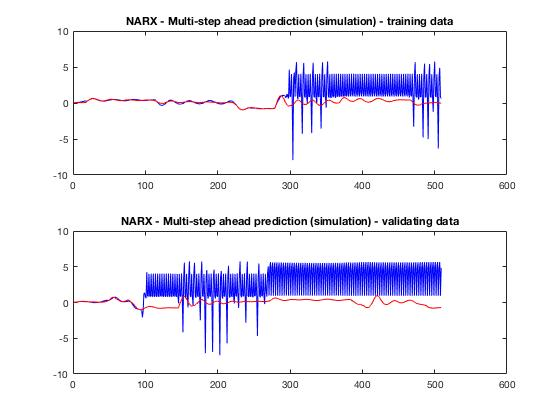
\includegraphics[width=0.75\textwidth, keepaspectratio]{10_simulation}
\caption{Symulacja rzeczywistego obiektu}
		\label{fig:10_simulation}
\end{figure}


Dla 100 neuronów w warstiwe ukrytej, 1000 epokach uczenia i opóźnieniem
wejść o 2 i wyjść o 3 na wejściu sieci otrzymałem wykresy przedstawione
na rysunku \ref{fig:100_one_step_ahead}
Wygenerowanie symulacji obiektu wynikające z zamknięcia pętli sprzężenia zwrotnego
zostało przedstawione na rysunku \ref{fig:100_simulation}.

\begin{figure}[H]
\centering
	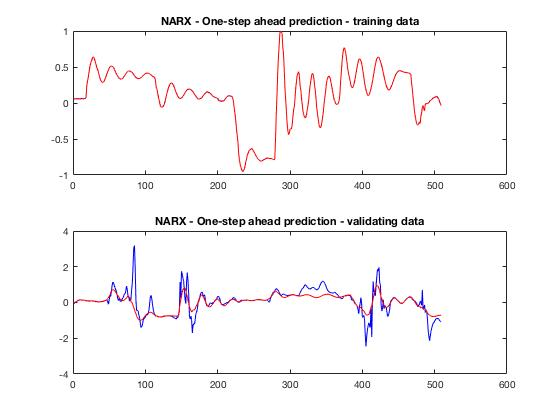
\includegraphics[width=0.80\textwidth, keepaspectratio]{100_one_step_ahead}
\caption{Wykresy predykcji one-step-ahead dla zbioru uczącego i walidacyjnego}
		\label{fig:100_one_step_ahead}
\end{figure}
\begin{figure}[H]
\centering
	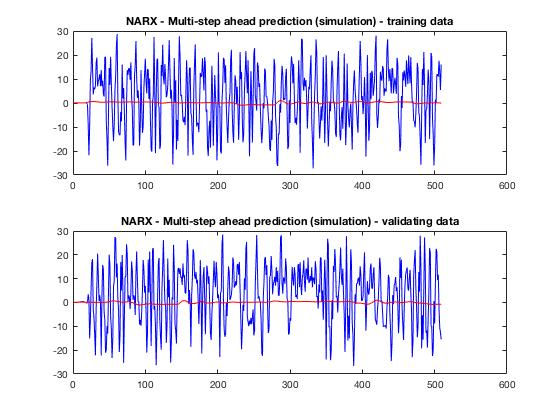
\includegraphics[width=0.75\textwidth, keepaspectratio]{100_simulation}
\caption{Symulacja rzeczywistego obiektu}
		\label{fig:100_simulation}
\end{figure}

Porównując otrzymane w ten sposób wyniki można stwierdzić, że zwiększenie ilości
neuronów w warstwie ukrytej nie zwiększa wydajności sieci. Po wynikach symulacji
obiektu przy użyciu modelu można stwierdzić, że zwiększenie ilości neuronów w warstwie
ukrytej powoduje większą czułość układu na zakłócenia. Układ rozpoczyna oscylacje
z dużą częstotliwością oraz wydaje się być łatwy do wyprowadzenia z równowagi.
Również właściwości predykcji one-step-ahead są gorsze dla modelu ze zbyt dużą ilością
neuronów w warstwie ukrytej.

W celu zbadania wpływu opóźnień na właściwości układu zmienione zostały parametry
opóźniające (konstruktor obiektu nnarx). Zmiana dotyczyła ilości opóźnień.
Żadna konfiguracja opóźnień nie dała lepszych wyników niż konfiguracja opóźnień
wyjść o 3 i wejść o 2.



\section{Wnioski}

Nieliniowe procesy są zwykle za bardzo skomplikowane dla modelowania tradycyjnymi
metodami statystycznymi. Modelowanie za pomocą nowoczesnych metod opierających
się o uczenie maszynowe czy sieci neuronowe pozwala na przybliżenie konkretnych
właściwości badanego układu. Nie pozwala jednak na pełną predykcję zachowań układu.
Należy zwrócić uwagę, że do właściwej identyfikacji systemu niezbędna jest duża
liczba danych i głębsza ich analiza. Sieć będzie się zachowywać tylko tak, jak
ją tego nauczymy i tylko na podstawie informacji, które zawarte były w danych
uczących.
W sprawozdaniu zostały opisane najprostsze scenariusze dotyczące działania
i modelowania rzeczywistych obiektów.
Modele wygenerowane za pomocą obiektu dedykowanego sieciom typu NNARX działały
znacznie szybciej i były prostsze w użyciu. Samo narzędzie dysponuje ogromną
ilością informacji na temat przebiegu uczenia, wartości wag czy właściwości
wygenerowanej sieci.
Sieci generowane ręcznie również służą jako dobry model dla sieci NNARX,
nie dają jednak tak dokładnej informacji o obiekcie.


\newpage
\begin{thebibliography}{9}

\bibitem{Osowski}
Stanisław Osowski.
\textit{Sieci Neuronowe w ujęciu algorytmicznym}
Wydawnictwo Naukowo-Techniczne, Warszawa 1996

\bibitem{strona}
Strona prowadzącego,
\\\texttt{http://staff.iiar.pwr.wroc.pl/piotr.ciskowski/skrypt/SNwMATLABie.htm}

\bibitem{springer}
J. Rhim, S. W. Lee
\textit{A neural network approach for damage detection and identification of structures}
Computational Mechanics, Springer 1995

\bibitem{springer}
Jerzy Lipski
\textit{Identyfikacja procesów dynamicznych z zastosowaniem sieci neuronowych}
Nauka i technika 2001

\end{thebibliography}


\end{document}
